
\section{Research Questions}
%%%%%%%%%%%%%%%%%%%%%%%%%%%%%%%%%%%%%%%%%%%%%%%%%%%%%%%%%%
\begin{frame}[t]
\begin{itemize}
	\item In the explicit approach, a finite numerical approximation of (often uncountably many) events in $\sa$s is required.
	\item Two primary sources of approximation error: 
	\begin{itemize}[<+->]
	
		\item (1) partitioning the parameter space $\pspace$ to approximate events in $\pborel$
		\item (2) partitioning the data space $\dspace$ to approximate events in $\BBB_{\dspace}$
	
	\end{itemize}
	\item A non-intrusive sample-based algorithm is initially introduced in \cite{BET+14} and further analyzed in \cite{BET+14-arxiv}
\end{itemize}
\end{frame}


%%%%%%%%%%%%%%%%%%%%%%%%%%%%%%%%%%%%%%%%%%%%%%%%%%%%%%%%%%
\begin{frame}[t]
\begin{itemize}
	\item <1-> Let $\PosxM$ be the exact solution to the approximate inverse problem using the discretization of $P_\dspace$ by $M$ samples
	\item <2-> Let $\PosxNM$ denote the approximate solution to the approximate problem under both aforementioned discretizations, so 
\[
\Pos = \lim\limits_{M\to\infty} \PosxM = \lim\limits_{M\to\infty} \lim\limits_{N\to\infty} \PosxNM
\]
	\item <3-> Let $\PosxNMh$ denote the approximate solution given the model discrepancy
\[
\PosxNM= \lim\limits_{h \downarrow 0} \PosxNMh
\]
\item <3-> $h$ refers to a mesh or other numerical parameter that determines the accuracy of the numerical solution evaluation of the QoI map
\end{itemize}

\end{frame}

%%%%%%%%%%%%%%%%%%%%%%%%%%%%%%%%%%%%%%%%%%%%%%%%%%%%%%%%%%
\begin{frame}[t]

Repeated application of the triangle inequality yields
\begin{equation}
\label{eq:triangleineq}
d_{\text{TV}}(\PosxNMh, \Pos) \leq 
\underset{ \text{(E1)} }{\underbrace{ d_{\text{TV}}(\PosxNMh, \PosxNM)}} + 
\underset{ \text{(E2)} }{\underbrace{ d_{\text{TV}}(\PosxNM, \PosxM) }}+ 
\underset{ \text{(E3)} }{\underbrace{ d_{\text{TV}}(\PosxM, \Pos) }}.
\end{equation}
\begin{itemize}

	\item <1-> The term (E1) describes the effect of the error in the numerically evaluated $Q_j$ on the solution to the stochastic inverse problem
	\item <2-> The term (E2) describes the effect of finite sampling error in $\pspace$, and (E3) describes the effect of discretization error of $P_\dspace$ on the solution to the stochastic inverse problem
	\item <3-> In our experience, terms (E1) and (E3) are more easily controlled
	\item <3-> Limit our focus to (E2), where certain geometric properties of the QoI map have an impact
\end{itemize}
\end{frame}

\subsection{Skewness and Accuracy}
%%%%%%%%%%%%%%%%%%%%%%%%%%%%%%%%%%%%%%%%%%%%%%%%%%%%%%%%%%
\begin{frame}[t]
\begin{itemize}
	\item In \cite{BGE+15}, the concept of \emph{skewness} in a QoI map $Q$ is introduced, quantified, and related to the accuracy in solving the stochastic inverse problem with a finite number of samples
	\item Geometric property that describes how the right angles in generalized rectangles belonging to $\dborel$ are transformed by $Q^{-1}$
\end{itemize}

\begin{defn}
For any QoI map $Q$, $\lambda \in \pspace$, and row vector $\bf{j}_k$ of Jacobian $J_{\lambda, Q}$, we define
\begin{equation}
S_Q(J_{\lambda,Q}, \bf{j}_k) := \frac{\abs{\bf{j}_k} }{\abs{\bf{j}_k^\perp}}.
\label{eq:skewness}
\end{equation}
We define the \textbf{local skewness} of a map $Q$ at a point $\pspace$ as 
\begin{equation}
S_Q(\lambda) := \max_{1\leq k \leq d} S_Q(J_{\lambda,Q}, \bf{j}_k).
\label{eq:localskewness}
\end{equation}
\end{defn}

\end{frame}

%%%%%%%%%%%%%%%%%%%%%%%%%%%%%%%%%%%%%%%%%%%%%%%%%%%%%%%%%%
\begin{frame}[t]
\begin{defn}
For any QoI map $Q$, $\lambda \in \pspace$, and row vector $\bf{j}_k$ of Jacobian $J_{\lambda, Q}$, we define
\begin{equation}
\begin{split}
S_Q(J_{\lambda,Q}, \bf{j}_k) &:= \frac{\abs{\bf{j}_k} }{\abs{\bf{j}_k^\perp}} \\
S_Q(\lambda) &:= \max_{1\leq k \leq d} S_Q(J_{\lambda,Q}, \bf{j}_k)
\end{split}
\end{equation}
\end{defn}

\begin{defn}
The \textbf{average} \emph{(or \textbf{expected})} \textbf{skewness} is defined as
\begin{equation}
\overline{S_Q} := \frac{1}{\mu_{\pspace}(\pspace)} \int_\pspace S_Q (\lambda) \, d\mu_{\pspace}
\label{eq:avgskew}
\end{equation}
\end{defn}

\begin{itemize}
	\item In \cite{BPW17}, it is shown that $S_Q(\lambda)$ is efficiently computed using SVDs of the Jacobian $J_{\lambda,Q}$
	\item In general, we approximate $\overline{S_Q}$ with Monte-Carlo approximations
\end{itemize}

\end{frame}




%%%%%%%%%%%%%%%%%%%%%%%%%%%%%%%%%%%%%%%%%%%%%%%%%%%%%%%%%%


%%%%%%%%%%%%%%%%%%%%%%%%%%%%%%%%%%%%%%%%%%%%%%%%%%%%%%%%%%
\begin{frame}[t]{A Simple Example: The Identity Map}
\vspace{-10pt}
\begin{figure}
	\begin{minipage}{.3\textwidth}
		\begin{itemize}
			\item $50$ samples
			\vskip 60pt
			\item $200$ samples
			\vskip 60pt
			\item $3200$ samples
		\end{itemize}
	\end{minipage}
	\begin{minipage}{.55\textwidth}
		\centering
    		$\Lambda$ \hskip 80pt $\mathcal{D}$
    		\vskip 0pt
    		\includegraphics[width=.5\textwidth]{images/finitesampling/approximate_input_50}
			\includegraphics[width=.5\textwidth]{images/finitesampling/approximate_output_50}\\
		\includegraphics[width=.5\textwidth]{images/finitesampling/approximate_input_200}
			\includegraphics[width=.5\textwidth]{images/finitesampling/approximate_output_200}\\
		\includegraphics[width=.5\textwidth]{images/finitesampling/approximate_input_3200}
			\includegraphics[width=.5\textwidth]{images/finitesampling/approximate_output_3200}\\
	\end{minipage}
\end{figure}

\end{frame}


%%%%%%%%%%%%%%%%%%%%%%%%%%%%%%%%%%%%%%%%%%%%%%%%%%%%%%%%%%
\begin{frame}[t]{Skewness}

\begin{figure}
    \begin{minipage}{.5\textwidth}
    	\centering
    	$\Lambda$
    	\vskip 0pt
    	\includegraphics[width=1\textwidth]{images/samemeasure_orthog}\\
    	\vskip 0pt
        %$\mu_\Lambda((Q^{(a)})^{-1}(B^{(a)})) = 0.0769$
    \end{minipage}%
    \begin{minipage}{.5\textwidth}
    \centering
    	$\Lambda$
    	\vskip 0pt
    	\includegraphics[width=1\textwidth]{images/samemeasure_skew}
        \vskip 0pt
    	%$\mu_\Lambda((Q^{(b)})^{-1}(B^{(b)})) = 0.0769$
    \end{minipage}
\end{figure}


\end{frame}

%%%%%%%%%%%%%%%%%%%%%%%%%%%%%%%%%%%%%%%%%%%%%%%%%%%%%%%%%%
\begin{frame}[t]{Numerical Approximation | Skewness}
\vspace{-10pt}
\begin{figure}
	\begin{minipage}{.3\textwidth}
		\begin{itemize}
			\item $50$ samples
			\vskip 60pt
			\item $200$ samples
			\vskip 60pt
			\item $800$ samples
		\end{itemize}
	\end{minipage}
	\begin{minipage}{.55\textwidth}
		\centering
    		$\Lambda$ \hskip 80pt $\Lambda$
    		\vskip 0pt
    		\includegraphics[width=.5\textwidth]{images/finitesampling/voronoi_symmdiff_orthog_50samples}
			\includegraphics[width=.5\textwidth]{images/finitesampling/voronoi_symmdiff_skew_50samples}\\
		\includegraphics[width=.5\textwidth]{images/finitesampling/voronoi_symmdiff_orthog_200samples}
			\includegraphics[width=.5\textwidth]{images/finitesampling/voronoi_symmdiff_skew_200samples}\\
		\includegraphics[width=.5\textwidth]{images/finitesampling/voronoi_symmdiff_orthog_800samples}
			\includegraphics[width=.5\textwidth]{images/finitesampling/voronoi_symmdiff_skew_800samples}\\
	\end{minipage}
\end{figure}

\end{frame}

%%%%%%%%%%%%%%%%%%%%%%%%%%%%%%%%%%%%%%%%%%%%%%%%%%%%%%%%%%
\begin{frame}[t]
\begin{example}
\label{ex:skewness}
Consider the following family of linear maps:
\begin{equation}\label{eq:qmap2}
\left \lbrace Q^{(s)} =  \mat{cc}{1 & 0 \\ \sqrt{s^2 - 1}& 1 } \right \rbrace_{s\in S},
\end{equation}
for $S=\set{1,2,4}$. 
\begin{itemize}
	\item Designed so the skewness of these maps is given by the index $s$, so $Q^{(1)}$ is $1$, the skewness of $Q^{(2)}$ is $2$, and $S_{Q^{(4)}} = 4$
	\item Preserves sizes of sets (determinant is one)
	\item Skewness has a direct impact on the number of samples required to achieve a given accuracy
	\item Provided a strong motivation for minimizing skewness and reinforces the results from \cite{BPW_2015}
\end{itemize}
\end{example}

\end{frame}


%%%%%%%%%%%%%%%%%%%%%%%%%%%%%%%%%%%%%%%%%%%%%%%%%%%%%%%%%%
\begin{frame}[t]
\small
\begin{figure}[h]
\begin{table}[H]
\begin{tabular}{ c | c | c | c }

N & $Q^{(a)}$ & $Q^{(b)}$ & $Q^{(c)}$\\ \hline \hline
$200$ & $2.97E-01$ & $3.42E-01$ & $5.28E-01$\\ \hline

$400$ & $2.00E-01$ & $2.41E-01$ & $3.79E-01$\\ \hline

$800$ & $1.59E-01$ & $1.78E-01$ & $2.88E-01$\\ \hline

$1600$ & $1.06E-01$ & $1.31E-01$ & $1.93E-01$\\ \hline

$3200$ & $8.38E-02$ & $9.39E-02$ & $1.41E-01$\\ \hline

$6400$ & $6.14E-02$ & $6.40E-02$ & $1.05E-01$\\ \hline

\end{tabular}
\end{table}

		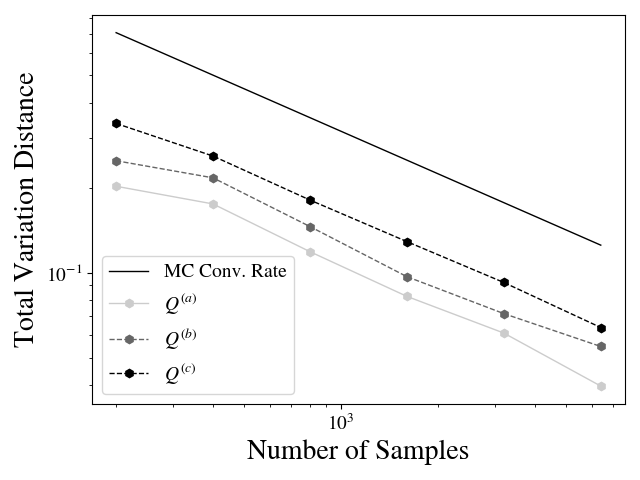
\includegraphics[width=0.5\linewidth]{./images/Plot-reg_BigN_40000_reg_M_1_rand_I_100000}

\caption{The results of $d_\text{TV}(\PosxNM, \PosxNN)$.}
\label{fig:skew}
\end{figure}
\end{frame}

%%%%%%%%%%%%%%%%%%%%%%%%%%%%%%%%%%%%%%%%%%%%%%%%%%%%%%%%%%
\subsection{Time Series Data}

%%%%%%%%%%%%%%%%%%%%%%%%%%%%%%%%%%%%%%%%%%%%%%%%%%%%%%%%%%
\begin{frame}[t]
\begin{itemize}[<+->]
	\item Let $t_0$ denote the initial time for the system being modeled 
	\item Let $\set{t_i}_{i=1}^M$ denote a set of observation times such that $t_0\leq t_1<t_2<\ldots<t_M$
	\item For each $1\leq i\leq M$, let $d_i$ denote the (noisy) measured (scalar) datum associated with some observable model output
	\item For each $1\leq i\leq M$, let $O_i(\lambda)$ denote the predicted value for $d_i$ obtained by solving the model for a particular $\lambda\in\pspace$
	\item We make a standard assumption used in the literature \cite{Smith, Barron, Silverman, Walpole} of an additive error noise model with independent errors $\eta_i$ for each $1\leq i\leq M$, i.e.
	\begin{equation}\label{eq:obs_data_error}
	d_i = O_i(\lambda) + \eta_i, \ 1\leq i\leq M,
\end{equation}
	\item We make the additional assumption that $\eta_i\sim N(0,\sigma_i^2)$ for each $1\leq i\leq M$.
\end{itemize}


\end{frame}

%%%%%%%%%%%%%%%%%%%%%%%%%%%%%%%%%%%%%%%%%%%%%%%%%%%%%%%%%%

%%%%%%%%%%%%%%%%%%%%%%%%%%%%%%%%%%%%%%%%%%%%%%%%%%%%%%%%%%
\begin{frame}[t]{Fundamental Questions}
\begin{itemize}[<+->]
	\item How do we construct a QoI map that incorporates all these observations?
	\item Should we treat observations as individual QoI in a vector-valued map or should we define a scalar-valued QoI map that incorporates all of the observations?
	\item Choosing a vector-valued approach will certainly introduce skewness effects into the QoI map, but doing this in an ``optimal'' way can reduce uncertainty~\cite{Walsh}.
	\item Choosing a scalar-valued approach that combines information across multiple observations will avoid skewness 
	\item Potentially at the cost of reducing the influence of potentially informative or sensitive observations on the posterior.
	\item Are some observations are more useful than others?
	\item Quantify utility of including less useful observations in the definition of the QoI map.
\end{itemize}

\end{frame}

%%%%%%%%%%%%%%%%%%%%%%%%%%%%%%%%%%%%%%%%%%%%%%%%%%%%%%%%%%
\subsection{Optimal Experimental Design - Questions and Considerations}
%%%%%%%%%%%%%%%%%%%%%%%%%%%%%%%%%%%%%%%%%%%%%%%%%%%%%%%%%%
\begin{frame}[t]
\begin{itemize}
	\item <1-> \emph{Quality of Measurements} -- Equipment with which we perform measurements introduces errors into the collected data.
	
	\item <2-> \emph{Duration of Experiment} -- Budgetary constraints, permits, access to equipment or space, and a host of other factors can influence the length of a given trial or experiment.
	
	\item <3-> \emph{Number of Trials} -- Can we achieve accuracy with fewer repetitions of an experiment?
	
	\item <4-> \emph{Measurement Frequency} -- How many measurements to take in each trial is directly related to the potential savings of shortening an experiment or reducing the number of repetitions necessary. 
	\item <4-> Is it better to temporally compress a fixed number of observations or space them out? 
	
	\item <5-> Can we potentially conduct shorter experiments that are equally informative to save time?
	\item <5-> Is it worth investing in something that is faster but less accurate? What are the trade-offs for precision and accuracy in the posterior?	
\end{itemize}

\end{frame}


%%%%%%%%%%%%%%%%%%%%%%%%%%%%%%%%%%%%%%%%%%%%%%%%%%%%%%%%%%
\begin{frame}[t]{Some More Considerations}
\begin{itemize}
	\item Current computational bottleneck is memory transfer and storage rather than processing speed.
	\item Questions of how to sift through data and pick out the most informative subsets of critical relevance to many scientists.
	\item If data are already collected, research is needed with respect to defining a QoI.
	\item There is a need for numerical studies investigating how information gain changes as more data are utilized.
	\item Subject of future investigation?
\end{itemize}
\end{frame}
